\noindent This appendix provides additional technical details on GUIWorld action representation, temporal alignment, and conditioning used in Section~\ref{section:impl-guiworld}.
Additional visualization pages are collected in Appendix~\ref{appendix:vis}; evaluation metrics and protocols are summarized in Appendix~\ref{appendix:gui-metrics}.

\subsection{Action schema}
\ncguiworld{} represents actions as a structured stream, enabling the NC to condition on both cursor movements and key presses.

At each timestep, we log absolute cursor coordinates, button up/down transitions, scroll deltas, and keyboard events.
Keyboard inputs are split into two types: typed characters (e.g., \texttt{ls -l}) and shortcut-style chords (e.g., \texttt{ctrl+v}).
We also track state flags such as whether a drag is currently active.
This lets us represent extended interactions like click-drag or press-hold as short labeled segments rather than isolated spikes.
The meta-action encoder described in Section~\ref{section:impl-guiworld} compresses this stream into a small typed schema.
In all reported v2 experiments, we use $S{=}2$ action slots per frame; empty slots are padded with type~0.
Each action has a type (e.g., \texttt{mouse click} or \texttt{keyboard type}) plus parameters.
Table~\ref{tab:meta-action-schema} summarizes the types and fields.
Type~0 corresponds to the absence of an action.
Type~1 encodes mouse clicks and drags via button identity, click count, and a drag flag.
Type~2 captures scrolls with a direction and scalar amount.
Type~3 packages free-form keyboard text (such as \texttt{ls -l}) embedded by the shared text encoder.
Type~4 records shortcuts such as \texttt{ctrl+v} via a small shortcut vocabulary.
This representation resembles a tool API while remaining recoverable from raw logs.

\begin{table}[h]
  \centering
  \small
  \setlength{\tabcolsep}{6pt}
  \renewcommand{\arraystretch}{1.05}
  \caption{Meta-action schema for GUIWorld (per action slot).}
  \label{tab:meta-action-schema}
  \rowcolors{2}{metablue!8}{white}
  \begin{tabularx}{\linewidth}{@{}c l >{\raggedright\arraybackslash}X@{}}
    \toprule
    \rowcolor{metablue!16}\textbf{Type id} & \textbf{Action} & \textbf{Parameter fields} \\
    0 & None & -- \\
    1 & Mouse Click/Drag & \texttt{button}, \texttt{click\_count}, \texttt{drag\_flag} \\
    2 & Mouse Scroll & \texttt{direction}, \texttt{amount} \\
    3 & Keyboard Type & \texttt{text} (e.g., \texttt{ls -l}) $\rightarrow$ shared text encoder \\
    4 & Shortcut & \texttt{shortcut\_id} (e.g., \texttt{ctrl+v}) \\
    \bottomrule
  \end{tabularx}
\end{table}

\subsection{Conditioning: encoders and injection}
The main text considers two encoders for this stream.
A \emph{raw-action encoder (v1)} keeps fine-grained mouse and key events in a multi-hot representation that closely mirrors real cursor and typing behavior.
A complementary \emph{meta-action encoder (v2)} compresses events into a small typed schema (Table~\ref{tab:meta-action-schema}) and embeds any free-form text with a shared text encoder.
Both encoders produce per-frame action features that undergo temporal windowing and alignment (described below).
These embeddings support four injection modes, summarized below:
\begin{tcolorbox}[
  colback=metablue!8,
  colframe=metablue!40,
  boxrule=0pt,
  borderline west={1pt}{0pt}{gray!60},
  left=6pt,right=4pt,top=3pt,bottom=3pt]
\small
\begin{itemize}
  \setlength{\itemsep}{2pt}
  \setlength{\topsep}{2pt}
  \item \texttt{external}: fuse actions at the VAE input.
  \item \texttt{contextual}: mix actions and frames as tokens in one sequence.
  \item \texttt{internal}: inject actions inside transformer blocks.
  \item \texttt{residual}: add lightweight action deltas to hidden states.
\end{itemize}
\end{tcolorbox}

\noindent\textbf{Injection-mode definitions (schematic)}
\label{appendix:gui-injection-equations}
Below we give compact schematic definitions for the three formula-based modes (\texttt{external}, \texttt{residual}, \texttt{internal}); \texttt{contextual} is specified by the structured attention mask in Figure~\ref{fig:contextual-mask}.
%
\textbf{External.} Given VAE latents $z_{1:T}$ and temporally aligned action features $u_{1:T}$, an external action module produces a residual update $\Delta z_{1:T}(u_{1:T})$ and forms modified latents
\[
  z'_{1:T} = z_{1:T} + \Delta z_{1:T}(u_{1:T}).
\]
The diffusion backbone then operates on $z'_{1:T}$ (actions do not appear as explicit tokens inside the transformer).
%
\textbf{Residual.} At selected transformer layers $l$, an auxiliary action module takes block hidden states $h^{(l)}$ together with local action/mouse features and outputs a residual update $\Delta h^{(l)}(a,\text{mouse})$.
The updated hidden states are
\[
  \tilde{h}^{(l)} = h^{(l)} + \Delta h^{(l)}(a,\text{mouse}),
\]
which are passed to the next block.

\textbf{Internal.} At selected blocks, action conditioning is inserted as an additional cross-attention sub-layer inside the standard attention stack.
With self-attention $\mathrm{SA}$, text/reference cross-attention $\mathrm{CA}_{\text{text}}$, and action cross-attention $\mathrm{CA}_{\text{action}}$, a schematic update is
\[
  h' = \mathrm{FFN}\Big(
    h + \mathrm{CA}_{\text{text}}\big(\mathrm{SA}(h), c\big)
      + \mathrm{CA}_{\text{action}}(h, a)
  \Big).
\]

\subsection{Temporal alignment and attention}
\noindent\textbf{Temporal alignment and windows.}
The GUI backbone processes a compressed latent video at stride $c$ (every $c$ pixel frames correspond to one latent frame).
For a pixel sequence of length $F$ and latent sequence of length $T$, we approximately have $F \approx (T-1)c + 1$ under uniform sampling.
Exact indexing follows the dataloader timestamp mapping and boundary handling.
Anchor frame $a_t = t \cdot c$ marks the pixel frame corresponding to latent step $t$.

Mouse and keyboard logs start as per-frame features $r_f \in \mathbb{R}^D$ at the pixel rate.
A windowed encoder aggregates them around each anchor over $p = c \cdot w$ frames.
Here $w$ controls the window width, and a lag $\ell$ accounts for GUI response delay (actions precede their visual effects).
We use zero-padding outside the valid range, i.e., $\tilde{r}_f=r_f$ for $0\le f<F$ and $\tilde{r}_f=0$ otherwise, and form a lag-shifted window that ends at $a_t-\ell$:
\[
  W_{t,k} = \tilde{r}_{\,a_t - (p-1+\ell) + k}, \quad k\in\{0,\dots,p-1\}, \quad
  a^{\text{act}}_t = \frac{1}{p} \sum_{k=0}^{p-1} W_{t,k}.
\]
This shared action encoder yields one latent-aligned action embedding $a^{\text{act}}_t$ per step.
It summarizes a short, lagged history of cursor motion and key events and is reused across all injection modes.

\noindent\textbf{Contextual attention mask.}
In the \texttt{contextual} mode, video and action tokens are concatenated into a single sequence and processed under a structured lag-aware local attention mask.
Appendix Figure~\ref{fig:contextual-mask} can be read as a query--key matrix: rows are queries and columns are keys.

The upper-left block (\emph{V2V}) restricts each frame $V_i$ to attend only to neighboring frames within a window of $\pm w$ steps, so very distant frames cannot interfere.
The upper-right block (\emph{V2A}) lets frame $V_i$ see only recent actions in a lag-bounded recent-action range.
In implementation, this window is $j \in [\max(0, i-\ell), \min(i, A-1)]$, where $\ell$ is the action lag and $A$ is the action-token length.
This way, frame conditioning stays focused on recent operations and excludes future actions.
In the lower-left block (\emph{A2V}), an action $A_i$ can attend to frames $V_t$ that occur after it has had time to take effect ($t \ge i+\ell$, with boundary clipping), but not to earlier frames.
This path is representation-only and does not expose future frame information to frame prediction.
The lower-right block (\emph{A2A}) is strict diagonal: each action token attends to itself.

In practice $(w,\ell)$ act as fixed hyperparameters that trade off temporal coverage and cost.
Together, these choices implement a structured lag-aware temporal prior: actions do not explain past frames, and each frame conditions on recent operations that could plausibly have shaped its pixels.

\noindent\textbf{Design insights.} Two insights from the GUI experiments motivate this schema.
First, raw action streams are bursty and high-dimensional.
Cursor and key events arrive in short spikes, and simple smoothing or full-history attention can cause false interpolated motion and underestimated typing speed.
Using short, lagged windows and local attention bands makes credit assignment more intuitive: each frame connects to the few operations that could have produced it.
Second, in our experiments, with the visual backbone fixed, control fidelity improved more from conditioning design than from encoder choice.
Clean, well-paced supervision and mid- or deep-level action injection improve cursor accuracy and hover timing, while different encodings of the same stream perform similarly.
This action schema and mask implement these principles: keep pixels and actions aligned in time, prioritize recent operations over distant ones, and use attention structure rather than~capacity~alone.

\subsection{Cursor rendering and supervision}
\noindent\textbf{Cursor rendering and reference construction.}
\label{appendix:cursor-rendering} 
%
The cursor pipeline applies the same design principles on the visual side.
Instead of relying on the global diffusion loss to recover a small, high-frequency visual target, we render the cursor explicitly.
We treat it as a first-class conditioning signal.

\noindent\textbf{From logs to normalized trajectories.}
\label{appendix:mouse-traj-normalization}
Desktop logs provide per-frame cursor positions in screen coordinates $(x_\text{screen},y_\text{screen})$ at the native GUI resolution.
We align these with sampled video frames using the same letterbox mapping as the RGB stream.
Given source and target resolutions $(w_\text{src}, h_\text{src})$ and $(w_\text{dst}, h_\text{dst})$, we compute a uniform scale $s$ and padding offsets $(p_x,p_y)$.
Each coordinate is then mapped to normalized positions $(x_t,y_t)\in[0,1]^2$ as
\[
  x_t = \frac{s\,x_{\text{screen},t} + p_x}{w_\text{dst}-1},\qquad
  y_t = \frac{s\,y_{\text{screen},t} + p_y}{h_\text{dst}-1}.
\]
Stacking these over time yields the trajectory tensor \texttt{mouse\_trajectories} used across rendering and action encoding.


\begin{table}[h!]
  \centering
  \small
  \setlength{\tabcolsep}{4pt}
  \renewcommand{\arraystretch}{1.12}
  \caption{Raw-action versus meta-action encoders in GUIWorld.}
  \label{tab:action-encoder-comparison}
  \begin{tabularx}{\linewidth}{p{2.9cm} >{\raggedright\arraybackslash}X >{\raggedright\arraybackslash}X}
    \toprule
    \textbf{Aspect} &
    \textbf{Raw-action encoder (v1)} &
    \textbf{Meta-action encoder (v2)} \\
    \midrule
    \textbf{Action schema} &
    Per-frame multi-hot vector composed of
    13 mouse actions and 169 keyboard actions;
    no explicit type hierarchy. &
    Hierarchical schema with explicit action types and parameters:
    \texttt{action\_types} $\in \{0,1,2,3,4\}$ for
    \{None, Mouse Click/Drag, Mouse Scroll, Keyboard Type, Keyboard Shortcut\},
    plus typed parameter fields (e.g., button, scroll amount, shortcut ID, text). \\[2pt]
    %
    \textbf{Mouse representation} &
    Two signals per frame:
    (1) continuous cursor trajectory
    $\texttt{mouse\_trajectories}_{t} \in \mathbb{R}^2$;
    (2) discrete mouse events
    $\texttt{mouse\_action\_events}_{t} \in \{0,1\}^{13}$ (multi-hot). &
    Per-frame mouse trajectory
    $\texttt{mouse\_trajectories}_{t}$
    is encoded by a shared mouse-trajectory encoder and the temporal windowing module into
    dense mouse embeddings
    $\texttt{mouse\_latent}_{t} \in \mathbb{R}^{d_{\text{mouse}}}$,
    optionally fused with action embeddings. \\[2pt]
    %
    \textbf{Keyboard representation} &
    Per-frame keyboard state
    $\texttt{keyboard\_action\_events}_{t} \in \{0,1\}^{169}$,
    where each dimension corresponds to a key or shortcut;
    only multi-hot activation is available, no text semantics. &
    Two complementary forms:
    keyboard shortcuts as
    \texttt{keyboard\_shortcut} IDs embedded via an embedding table, and
    free-form text \texttt{keyboard\_text} (e.g.\ ``ls -l'')
    encoded by a shared text encoder (e.g., T5) and projected to the
    action embedding dimension. \\[2pt]
    %
    \textbf{Per-frame representation} &
    Mouse and keyboard events are concatenated:
    $\texttt{raw\_actions}_{t}
      = [\,\texttt{mouse\_events}_{t},\,
           \texttt{keyboard\_events}_{t}\,]
      \in \mathbb{R}^{182}$. &
    For each frame $t$ and slot $s$,
    type plus parameters are embedded into
    \texttt{slot\_embeds}$_{t,s} \in \mathbb{R}^{D}$.
    Valid slots are aggregated (mean or attention) into a single
    per-frame action embedding
    $\texttt{action\_embeds}_{t} \in \mathbb{R}^{D}$. \\[2pt]
    %
    \textbf{Multi-slot support} &
    No explicit notion of multiple action slots per frame;
    all mouse and keyboard signals are collapsed into one
    182-d multi-hot vector. &
    Explicit multi-slot design:
    \texttt{action\_types} and all parameter tensors have shape
    $(B, T, S)$ with $S=2$ slots per frame,
    enabling, e.g., concurrent ``mouse click + keyboard shortcut''
    in the same frame. \\[2pt]
    %
    \textbf{Latent-aligned representation} &
    Temporal alignment is implemented ad-hoc inside each
    v1 action module (e.g., sliding windows over the
    182-d per-frame vector),
    with custom logic per mode (external, internal, residual). &
    A unified temporal alignment module takes per-frame action embeddings
    $(B, F, D)$ and VAE compression ratio $c$,
    constructs lag-aware temporal windows of size
    $c \cdot w$,
    and outputs latent-aligned action features
    $\texttt{action\_latent} \in \mathbb{R}^{B \times T \times D}$,
    with analogous $\texttt{mouse\_latent}$ when mouse features are enabled. \\[2pt]
    %
    \textbf{Lag modeling} &
    GUI latency / response lag is implicitly encoded
    by where and how the sliding window is applied
    inside each v1 action module; there is no shared
    lag configuration across modes. &
    Lag is an explicit hyperparameter
    \texttt{action\_lag} in the temporal alignment and in
    the contextual attention mask:
    it shifts temporal windows and defines which frames
    an action can attend to, giving a consistent lag interpretation across modes. \\[2pt]
    %
    \textbf{Downstream usage} &
    Raw 182-d vectors (plus trajectories) are fed directly into the v1 action modules (external, internal, residual) without a shared temporal encoder. &
    The v2 encoder outputs provide a shared conditioning stream for all v2 modes and also supply features for the temporal contrastive loss. \\[2pt]
    %
    \textbf{Contrastive supervision} &
    No dedicated temporal contrastive loss between frames
    and actions; supervision comes only from the generative objective. &
    Action and mouse latents are coupled to frame features via
    an InfoNCE-style temporal contrastive loss, encouraging time-aligned action embeddings. \\
    \bottomrule
  \end{tabularx}
\end{table}


\subsection{Training signals and encoder design}

\noindent\textbf{From trajectories to cursor layers.}
Starting from normalized $(x_t,y_t)$ coordinates, a cursor-layer module renders a fixed SVG arrow template into RGB and alpha channels.
The template is reused across frames.
For each timestep $t$, it is positioned so the hotspot (arrow tip) aligns with $(x_t,y_t)$, clipped to screen bounds, and alpha-blended over a neutral background.
This produces two tensors at video frame rate: a cursor-only foreground image $f_t \in [-1,1]^{3\times H \times W}$ and a soft mask $m_t \in [0,1]^{1\times H \times W}$ isolating the arrow pixels.
Invalid or missing coordinates zero the mask and leave the foreground unchanged, so frames without visible cursors do not add spurious supervision.

\noindent\textbf{Reference images and masks.}
These cursor layers become reference conditions for the image-to-video (I2V) model.
For each clip we form reference images $\mathrm{ref\_img}_{0:T-1}$ and masks $\mathrm{ref\_mask}_{0:T-1}$:
\begin{itemize}
  \item At $t{=}0$, $\mathrm{ref\_img}_0$ is the full desktop frame and $\mathrm{ref\_mask}_0$ is all ones, anchoring the static layout and theme;
  \item For $t{>}0$, $\mathrm{ref\_img}_t$ is the cursor foreground $f_t$ and $\mathrm{ref\_mask}_t$ is the cursor mask $m_t$, so only the arrow region is supervised while the background remains free.
\end{itemize}
The model encodes these references with the same VAE as target frames and concatenates their latents and masks into the diffusion input.
It enforces masked, reference-consistent reconstruction inside the cursor region while relying on learned dynamics elsewhere.
This makes cursor supervision a pixel-level constraint rather than a side effect of the global loss.

\noindent\textbf{Fourier mouse encoding.}
The same $(x_t,y_t)$ trajectories serve as a continuous control signal.
We apply a Fourier position module: clamp coordinates to $[0,1]^2$, map them to $[-1,1]^2$, and compute random Fourier features via a fixed Gaussian projection followed by sine/cosine.
A small MLP maps these features to per-frame mouse embeddings.
The GUIWorld action encoder then aggregates them with lag-aware, stride-aligned windows to produce latent-aligned mouse features.
These features condition the \texttt{external}/\texttt{contextual}/\texttt{residual}/\texttt{internal} modes and participate in the temporal contrastive loss.

\noindent\textbf{Cursor-aware losses.}
Section~\ref{section:impl-guiworld} introduces cursor-aware losses that use this construction.
A basic variant penalizes position error only in $(x,y)$.
Richer variants add Fourier features of the trajectory and, most importantly, an $\ell_2$ loss on the reconstructed cursor patch under $\mathrm{ref\_mask}_t$.
Table~\ref{tab:cursor-loss} shows that position-only objectives yield low cursor hit rate and visibly jittery arrows even when videos look plausible.
Adding the explicit cursor reference stream together with the masked patch loss substantially improves control, reaching 98.7\% cursor accuracy.
This confirms that explicit cursor rendering plus localized supervision effectively separates ``where the arrow is'' from ``what the rest of the frame should look like''.

\noindent\textbf{Temporal contrastive alignment.}
To strengthen learning signals for the action pathway, we add a lightweight temporal contrastive loss that operates on the same latent timeline as the diffusion model.
For each sequence we take per-step frame features $F_{t} \in \mathbb{R}^{d_f}$ pooled from the latent video.
We also take per-step action features $A_{t} \in \mathbb{R}^{d_a}$ and (optionally) mouse features $M_{t} \in \mathbb{R}^{d_m}$ produced by the action encoder.
Linear projections map these into a common space and the resulting vectors are $\ell_2$-normalized.
An InfoNCE-style objective brings matching pairs $(F_t,A_t)$ (and, when present, $(F_t,M_t)$) from the same timestep together.
In implementation, matching is lag-aware: frame $t$ is aligned with action/mouse features at $t-\ell$, where $\ell$ is the configured \texttt{action\_lag}.
Similarities are scaled by a temperature $\tau$.
It pushes matched pairs away from other timesteps of the \emph{same} sequence.
We use frame and action masks to ignore positions without actions.
A symmetric variant averages frame-to-action and action-to-frame directions.

When enabled, a small future-prediction head adds a second term.
Action features at time $t$ are mapped to a prediction of the frame feature at a slightly later step $t+\ell$.
A mean-squared error encourages consistency between the prediction and the projected future frame.
Together, these terms give the action encoder direct gradients tied to specific frames rather than relying solely on the pixel diffusion loss.
The contrastive term enforces tight temporal alignment between actions and the frames they co-occur with.
The future head encourages actions to anticipate the visual consequences that appear shortly after they are issued.


\noindent\textbf{Encoder comparison.}
Table~\ref{tab:action-encoder-comparison} contrasts the two encoders used in GUIWorld.
The key theme is moving from a high-dimensional, bursty event vector toward a typed, API-like schema with explicit lag handling.
This makes the action stream easier to align with the latent video timeline and to reuse across injection modes.



\begin{figure}[t]
  \centering
  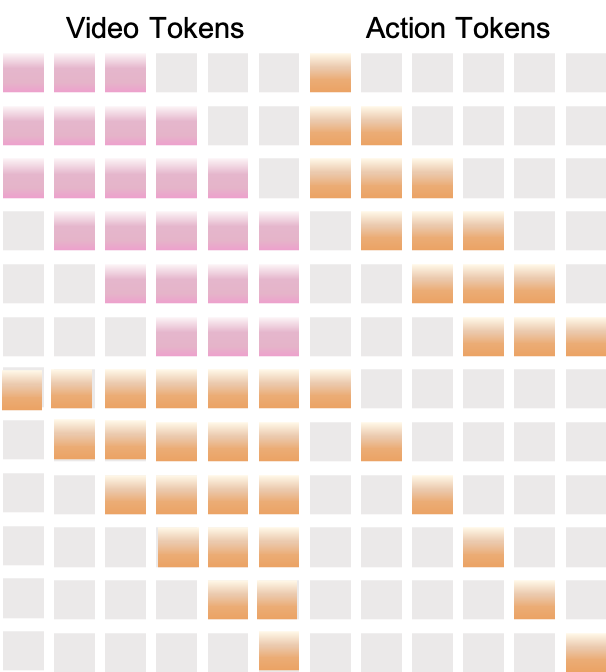
\includegraphics[width=0.5\linewidth]{assets/contextual_mask2.png}
  \caption{Contextual attention mask for GUIWorld.
  Video tokens (pink) and action tokens (orange) share one sequence.
  The mask restricts attention to a short temporal window so each frame attends only to nearby frames and temporally aligned actions.}
  \label{fig:contextual-mask}
\end{figure}

\noindent\textbf{Injection schemes.}
The GUI experiments explore four conditioning schemes built on this encoder: \texttt{external}, \texttt{contextual}, \texttt{internal}, and \texttt{residual} (Figure~\ref{fig:action-injection}).
Representative action-driven metrics comparing these modes are reported in Table~\ref{tab:gui-action-ssim}.
Full metric definitions and the evaluation protocol are provided in Appendix~\ref{appendix:gui-metrics}.
